\section{Poświęcenie palm i procesja}

\begin{itemize}
	\item w tej części \dd~ wykonuje pocałunki \ii~ standardowo jak podczas mszy
	\item podczas ubierania (na {\color{red} czerwono}) celebransa asystuje \cc,
	      kolejno diakona \aa1 oraz subdiakona \aa2
	\item ustawiamy się w szyku procesyjnym. \dd~ i \ss~ przez cały czas
	      procesji i poświęcenia ,jeżeli jest to możliwe, trzymają kapę.
	      Wychodzimy przez główne wyjście na zewnątrz. Przy przechodzeniu przez
	      oś ołtarza polowego, przyklękają wszyscy oprócz: \ding{63}, \aa1, \aa2
	      oraz \ii
	\item schola śpiewa podczas procesji \textit{Hosanna filio David} na
	      przemian z Psalmem 117 \footnote{Zob. \textit{Liber Usualis} z 1961 :
		      Ritus servandus in celebratione Missae in Cantu ad 1.}
	\item po dojściu na miejsce święcenia palm, \cc~ odbiera nakrycia głowy,
	      następuje  oddanie referencji ołtarzowi przez \dd~ i \ss~ oraz \ii~
	      (\dd~ i \ss~ przyklękają, \ii~ głęboko się skłania), \ii~ całuje
	      ołtarz następnie ustawiamy się w sposób przedstawiony na Rys.
	      \ref{fig:przyjscie}

	      \begin{figure}[h]
		      \centering
		      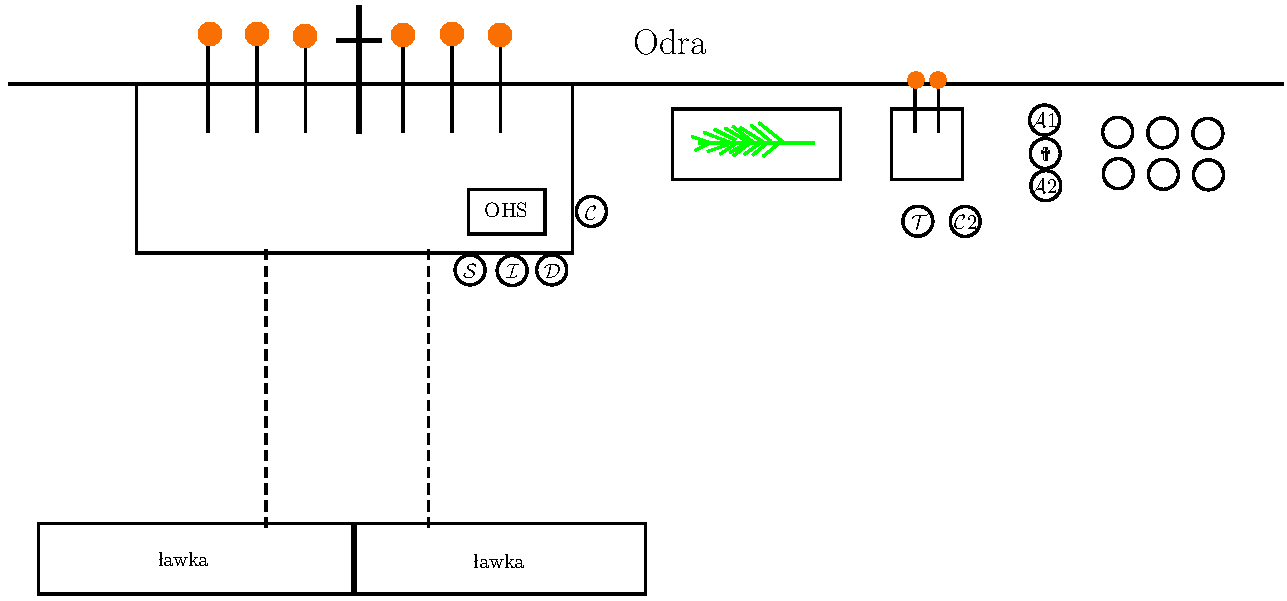
\includegraphics[width=0.8\linewidth]{Palmowa/PalmyNadOdra.pdf}
		      \caption{Ustawienie po przyjściu do ołtarza}
		      \label{fig:przyjscie}
	      \end{figure}

	\item \ii~ cicho odczytuje antyfonę \textit{Hosanna filio David}, tak jak
	      podczas Mszy, a następnie śpiewa \textit{Dominus vobiscum}, zwrócony w
	      kierunku księgi
	\item po \textit{Amen} następuje zasypanie
	\item \aa1 podaje wodę \cc~ a ten podaje ją \dd
	\item następuje pokropienie, \aa1 odbiera wodę od \dd
	\item następuję okadzenie
	\item palmę dla \ii~ \dd~ kładzie na ołtarzu
	\item następuje rozdawanie palm (\cc2 podaje palmy, \cc1 zawiaduje ruchem),
	      odbieranie palm od \ii~ i \dd~ z pocałunkiem, asysta ustawia się
	      dwójkami jak do komunii w kolejności: \dd~ i \ss~, klerycy,
	      ministranci, lud
	\item po rozdaniu palm \ii~ i \dd~ myją ręce, pomagają mu w tym \aa\aa
	\item następuje odśpiewanie ewangelii, nie przenosi się mszału
	\item do ewangelii ustawiamy się jak podczas mszy, gdy już dojdziemy na
	      miejsce jak na Rys. \ref{fig:ewangelia}

	      \begin{figure}[h!]
		      \centering
		      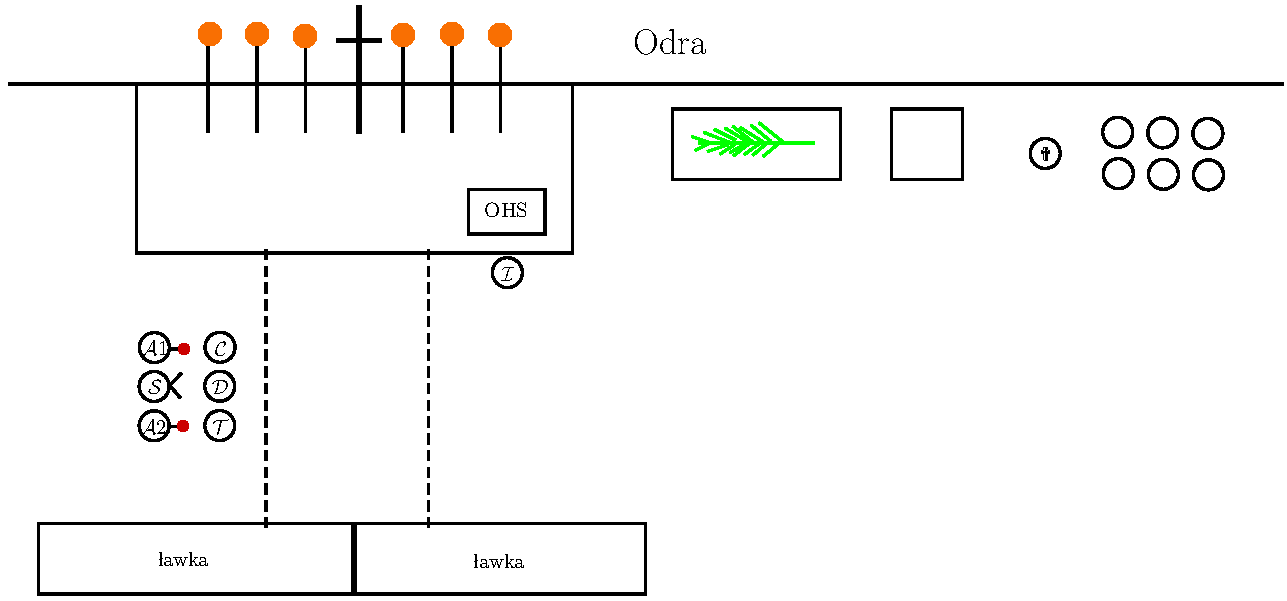
\includegraphics[width=0.8\linewidth]{Palmowa/PalmyNadOdra2.pdf}
		      \caption{Ustawienie podczas Ewangelii}
		      \label{fig:ewangelia}
	      \end{figure}

	\item po odśpiewaniu ewangelii \ii~ całuje ewangeliarz oraz jest okadzany
	      przez \dd
	\item kantorzy ($K1$) oraz mikrofoniarz udają się najkrótszą możliwą drogą
	      do pierwszych drzwi kościoła. Przymykają je lekko, ale obserwują, czy
	      procesja już się zbliża. Dwóch lub jeden kantor ($K2$) pozostaje w
	      procesji z ministrantami
	\item po powrocie do pozycji z Rys. \ref{fig:przyjscie} następuje zasypanie
	\item \dd~ i \ss~ stają w rzędzie za \ii
	\item \dd~ staje obok rzędu i śpiewa \textit{Procedeamus in pace}
	\item kantor ($K2$) oraz mikrofon wraz z ludem śpiewa \textit{In nomine
		      Christi. Amen}, a następnie rozpocznie jedno z poniższych:

	      \begin{itemize}
		      \item śpiew jednej z antyfon procesyjnych z \textit{Liber
			            Usualis}
		      \item \textit{Christus vincit}
		      \item pieśń po polsku do Chrystusa Króla
	      \end{itemize}

	\item po oddaniu rewerencji ołtarzowi \cc~ oddaje nakrycia głowy
	\item ustawiamy się w szyku procesyjnym, $K2$ zajmują w procesji miejsce
	      zaraz za \ding{63}
	\item udajemy się w kierunku bocznych drzwi po schodach za pomnikiem biskupa
	      Kominka
	\item $K1$ wewnątrz kościoła obserwują delikatnie, czy procesja nadchodzi
	\item kiedy procesja dochodzi do drzwi kościoła, \ss~ z \aa\aa~ stają przodem
	      do drzwi, a ministranci rozchodzą się na boki tworząc szpaler tak aby
	      \ii~ znajdował się nieopodal \ding{63}, jak na Rys. \ref{fig:procesja}

	      \medskip

	      \begin{figure}[h]
		      \centering
		      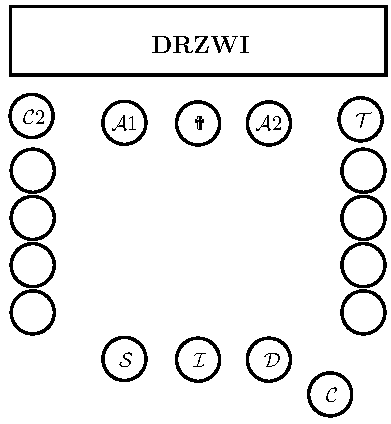
\includegraphics[width=0.26\linewidth]{Palmowa/PalmyNadOdra3.pdf}
		      \caption{Procesja przy drzwiach kościoła}
		      \label{fig:procesja}
	      \end{figure}
	      \todo{A gdzie mają być ci kantorzy na tym rysunku?}

	\item $K1$ (w środku) stojąc zwróceni w kierunku drzwi śpiewają:
	      \textit{Gloria Laus et honor} etc.
	\item $K2$, ministranci i wierni powtarzają werset: \textit{Gloria Laus}
	\item $K1$ śpiewają poszczególne zwrotki hymnu, po każdej zwrotce
	      $K2$ i reszta odśpiewują refren: \textit{Gloria, Laus}
	\item po piątej zwrotce i refrenie \ding{63} głośno i widocznie uderza nóżką
	      krzyża procesyjnego w drzwi, a $K1$ i \cc2 szeroko otwierają drzwi
	\item \cc2 wprowadza \ding{63} i resztę procesji do wnętrza kościoła. W tym
	      czasie $K1$ i $K2$ łączą się w jedną grupę i jak najszybciej zaczynają
	      śpiew: \textit{Ingrediente Domino}, podany w
	      \textit{Liber Usualis}
	\item \dd, \ss, \ii~ oraz \cc~ po przyklęknięciu na środku udają się
	      bezpośrednio do księgi po stronie epistoły, reszta asysty i chór
	      przyklękają po kolei na środku. Wszyscy zajmują swoje miejsca i
	      odkładają palmy. \aa\aa~ odkładają świece a \ding{63} krzyż na stojak
	\item modlitwa na zakończenie procesji od Mszału ustawionego przy ołtarzu po
	      stronie Epistoły, \dd~ i \ss~ trzymają brzegi kapy (jak przy poświęceniu)
	\item po skończonej oracji, \ii~ i \dd~ oraz \ss~ podchodzą do sedilli i
	      przebierają się (w {\color{violet}fiolety}). Przebieranie przebiega w
	      następującej kolejności:

	      \begin{itemize}
		      \item \cc~ zabiera kapę przekazuje \zz
		      \item \dd~ i \ss~ ściągają dalmatyki z pomocą \aa1 oraz \aa2
		      \item \cc~ ubierają w ornat \ii, \zz~ zabierają w tym
		            czasie dalmatyki i manipularze czerwone
		      \item \aa1 zakłada tunicelę \ss, \aa2 dalmatykę \dd
		      \item \cc~ sprawdza czy \dd~ i \ss~ mają odpowiednie szaty
	      \end{itemize}

	\item w czasie przebierania schola śpiewa \textit{Introit}
\end{itemize}